
\section{Numerical Experiments}
This section is organized as follows. The first part is dedicated to the numerical implementation
of the frequency domain formulation \eqref{eq:main_frequency_domain}. We study the convergence of this formulation and the behaviour 
of the numerical solution as the absorption parameter $\nu$ tends to zero. The experiments in this section were 
performed with the help of \urev{our} code written in Octave.  
We implemented the scheme described in Section \ref{sec:discr} for a case of $P_{1}$-space used 
for the approximation of $E_{x}$ and $E_{y}$ and $\theta=0$, thus working with the system (\ref{eq:simple_system}). 
We apply permutation to the above system 
to obtain a 7-diagonal Hermitian matrix and solve the system with the Gauss back substitution algorithm. 

The intermediate part briefly validates the semi-lagrangian discretization of the time domain formulation.

The last part of the section deals with the question of the equivalence of the limiting absorption and limited amplitude 
principle. We compare the solutions obtained as $\nu\rightarrow 0$ with the help of \mrev{the frequency   
and time domain codes }(computed for large values of time). 
The time-domain code implements the scheme described in \urev{Section \ref{sec:staggered_discretization}} and 
is written in Fortran.
 
\subsection{Frequency Domain Problem}
\label{sec:freq_dep}
\subsubsection{Validity of the Implementation}
\label{sec:airy_fd_validity}
To check the validity of the code, we first perform a numerical experiment with (formally chosen) parameters:
\begin{align}
\label{eq:parameters}
\alpha(x)=x^2+1,\qquad \delta(x)=\left(\alpha^2+x\alpha\right)^{\frac{1}{2}}, \qquad \mrev{\nu=0, \qquad \theta=0.}
\end{align}
\urev{It can be shown that $E_{y}$ that solves (\ref{eq:main_frequency_domain}) with the above parameters,  
and $\nu=0$, satisfies the Airy equation, see also Remark \ref{remark:other},
\begin{align*}
 E_y''-xE_y=0,\qquad x\in [-L,\; H].
\end{align*}
One of the solutions of this equation, an Airy function \urev{$\Ai(x)$}, see \cite[Chapter 10.4]{abramowitz_stegun}, is analytic and 
decays rapidly as $x\rightarrow \infty$. }
\mrev{Hence, choosing $H$ sufficiently large (the actual value used in the experiments $H=10$, where $\left|\Ai'(10)\right|<1e-9$) and the boundary conditions as 
\begin{align}
\label{eq:bcs_airy}
\partial_{1}E_{y}(-L)+2iE_{y}(-L)=2i\Ai(-L)+\Ai'(-L),\qquad 
\partial_{1}E_{y}(H)=0\approx \Ai'(H),
\end{align}
where $\Ai(x)$ is an Airy function, we ensure that $E_{y}$ that solves the above problem is well approximated by $\Ai(x)$, and $E_{x}$ by $-i\frac{\delta(x)}{\alpha(x)}\Ai(x)$. 
The well-posedness of the respective variational formulation for $\nu=0$ is due to Remark \ref{remark:other}. }

In Fig.~\ref{fig:conv_rate} we demonstrate the convergence rates for this problem, comparing the solution with the 
known analytic solution. 
Importantly, the obtained convergence rates are in agreement with known estimates of the standard theory of convergence~\cite[Chapter 5.7,
Chapter 0.4]{brenner}, \mrev{provided that the Aubin-Nitsche lemma \cite[Theorems 3.2.4,3.2.5]{ciarlet_fem} holds for the variational formulation.}  
\begin{figure}
\begin{tikzpicture}
    \begin{loglogaxis}[
        xlabel=$h$,
        ylabel=$Error$,
        width=0.4\textwidth,
        xmin=2e-6,
        ymin=1e-8,
        xmax=2,
	legend cell align=left,
        legend style={
at={(1.7,0.5)},
%legend pos=outer north east, 
anchor=east,
%legend pos=south east,
%anchor=east, 
draw=none,
font=\small
}
]\addplot[mark=*,black] table {pics_frequency_domain/data_airy/E1L2.dat}; 
    \addlegendentry{$\|E_{x}-E_{x}^{c}\|_{L^2}$};
    \addplot[mark=*,red, mark size=1pt] table {pics_frequency_domain/data_airy/E2H1.dat};
        \addlegendentry{$\|E_{y}-E_{y}^{c}\|_{H^{1}}$};
        
          \addplot[mark=*,cyan, mark size=1pt] table {pics_frequency_domain/data_airy/E2L2.dat};
        \addlegendentry{$\|E_{y}-E_{y}^{c}\|_{L^{2}}$};  
        \addplot[dotted] table{pics_frequency_domain/data_airy/E_h2.dat};
         \addlegendentry{$O(h^2)$};
         \addplot[dashed] table{pics_frequency_domain/data_airy/H.dat};
         \addlegendentry{$O(h)$};
    \end{loglogaxis}
    \end{tikzpicture}
    \caption{Convergence rates for the \mrev{problem described in Section \ref{sec:airy_fd_validity} (the problem (\ref{eq:main_frequency_domain}) discretized as (\ref{eq:simple_system})} 
    with the parameters (\ref{eq:parameters}) and the \mrev{boundary condition (\ref{eq:bcs_airy}))}. \mrev{Here $E_{y}^{c}(x)=\Ai(x)$ and 
    $E_{x}^{c}(x)=-i\frac{\delta(x)}{\alpha(x)}\Ai(x)$.}}
    \label{fig:conv_rate}
\end{figure}
\subsubsection{Solution of a Frequency-Domain Problem with Resonance}
%\paragraph{Convergence}
Let us consider the case of the resonance, more precisely, we choose sufficiently smooth
$\alpha,\delta$, s.t. $\alpha(0)=0$ and $\delta(0)\neq 0$, and the solvability conditions 
of Lemma \ref{lemma:well_posedness}  are satisfied. 
For simplicity, let us assume 
\begin{align}
\label{eq:cond}
 \alpha(x)=-x \text{  in some neighbourhood of $0$ }.
\end{align}
\mrev{Let $h>0$ denote the meshwidth. }Given $\mathbf{V}_{h}=P_{h}^{1}\times P_{h}^{1}$, with $P_{h}^{1}$ consisting of piecewise-linear (hat) functions, 
\mrev{and $E^{\nu}_{x},\;E^{\nu,h}_{x}$ being correspondingly the exact and the numerical solution, }
we look for a ratio $h(\nu)$ that would ensure the bound on the absolute error 
\begin{align}
\label{eq:problem1}
\|E^{\nu}_{x}-E^{\nu,h}_{x}\|_{L^2}<\epsilon,
\end{align}
given a fixed value of $\epsilon>0$ and $\nu\rightarrow 0$. W.l.o.g. here we assume that $\nu>0$. 

We use the following ingredients:
\begin{itemize}
 \item The C\'ea's lemma applied to the problem (\ref{vf1dcase}); here \mrev{$\mathbf{E}^{\nu}$ is the exact solution, 
 $\mathbf{E}^{\nu,h}$ is the computed solution}, and $C_c$ is the continuity and $C_i$ is the coercivity constants:
\begin{align}
\label{eq:cea}
\begin{split}
 \|\mathbf{E}^{\nu}-\mathbf{E}^{\nu,h}\|_{\mathbf{V}}\leq \frac{C_c}{C_i}\min_{\mathbf{v}\in \mathbf{V}_h}\|\mathbf{E}^{\nu}-\mathbf{v}\|_{V}
 \leq C\nu^{-1}\min_{\mathbf{v}\in \mathbf{V}_h}\|\mathbf{E}^{\nu}-\mathbf{v}\|_{\mathbf{V}},\; C>0.
 \end{split}
\end{align}
The last inequality follows from Lemma \ref{lemma:well_posedness} and is valid for $\nu\rightarrow 0$.   
\item The form of the exact solution to the problem (\ref{vf1dcase}), see \cite{Despres_2014},
\begin{align}
\label{eq:exact}
 E_x^{\nu}=-iE_{y}^{\nu}\frac{\delta}{\alpha+i\nu}=\frac{f^{\nu}(x)}{\alpha(x)+i\nu}, \; \text{for some }f^{\nu}(x)\in L^2(\Omega).
\end{align}
\item \mrev{An explicit bound on $\|\left(E_{y}^{\nu}\right)''\|_{L^{2}(\Omega)}$ based on the results of \cite{singular_solutions}. First of all, we
will assume that the main contribution to $\|\left(E_{y}^{\nu}\right)''\|_{L^{2}(\Omega)}$ comes from the behaviour in the vicinity of the point of the resonance, where 
the following expansion is valid \cite[Proposition 1]{singular_solutions}
\begin{align*}
E_{y}^{\nu}(x)=\tilde{E}_{y}^{\nu}(x)+S_{\nu}(x), \\
\tilde{E}_{y}^{\nu}(x)=\log\rho_{\nu}(x-X_{\nu})(\alpha(x)+i\nu)p_{\nu}(x),
\end{align*}
where $\rho_{\nu}$ is a smooth function s.t. $\rho_{\nu}(0)=0,\; \rho_{\nu}'(0)\neq 0$, the point $X_{\nu}\approx i\nu c+O(\nu^2)$, for some $c\in\mathbb{R}$, 
and $p_{\nu}(x),\; S_{\nu}(x)$ are smooth functions, which, together with their derivatives, are bounded independently of $\nu$.}
\item The estimate from \cite[Chapter 0]{brenner} on the rate of convergence of the interpolation 
\begin{align}
\label{eq:interp}
\begin{split}
 \|v-I^{h}v\|_{L^2}\leq Ch^2\left|v''\right|_{L^2},\; C>0,\\
 \|v-I^{h}v\|_{H^1}\leq Ch|v''|_{L^2},\; C>0, 
 \end{split}
\end{align}
where $I^{h}v$ is an interpolation operator onto $P_{h}^{1}$. 
\end{itemize}
The estimate (\ref{eq:cea}) combined with (\ref{eq:interp}) results in, for some $C>0$,
\begin{align}
  \label{eq:final_est}
  \|E^{\nu}_{x}-E^{\nu,h}_{x}\|_{L^2}%\leq C_1\nu^{-1}h\|\left(E_y^{\nu}\right)''\|_{L_{2}}+C_2\nu^{-1}h^2\|\left(E_x^{\nu}\right)''\|_{L_{2}}
  \leq C\nu^{-1}h\|\left(E_y^{\nu}\right)''\|_{L^2}+C\nu^{-1}h^2\|\left(E_x^{\nu}\right)''\|_{L^2}.
\end{align}
\mrev{
First of all let us examine the behaviour the derivatives of $E_{y}^{\nu}$ in the vicinity of the resonance:
\begin{align}
\label{eq:eynuprime}
 \left(\tilde{E}_{y}^{\nu}\right)'&=\frac{\alpha(x)+i\nu}{\rho_{\nu}(x-X_{\nu})}p_{\nu}(x)+\alpha'\log\rho_{\nu}(x-X_{\nu})p_{\nu}(x)+p'_{\nu}(x)(\alpha+i\nu)\log\rho_{\nu}(x-X_{\nu}).
\end{align}
The first term in the above expression is well-defined in $x=0$, even for $\nu=0$ (the limit can be obtained with the help of the L'Hopital's rule), and is uniformly bounded in $\nu$, together with its derivatives. The same holds for the third term. To examine the behaviour of $\left(\tilde{E}_{y}^{\nu}\right)''$, we study solely the singular second term of (\ref{eq:eynuprime})
\begin{align*}
 \left(\alpha'\log\rho_{\nu}(x-X_{\nu})p_{\nu}\right)'=\alpha''\log\rho_{\nu}(x-X_{\nu})p_{\nu}+\frac{\alpha'p_{\nu}}{\rho_{\nu}(x-X_{\nu})}\rho'_{\nu}(x-X_{\nu})+
 \alpha'\log\rho_{\nu}(x-X_{\nu})p_{\nu}'.
\end{align*}
The most singular term in the above expression is $\frac{\alpha'p_{\nu}}{\rho_{\nu}(x-X_{\nu})}\rho'_{\nu}(x-X_{\nu})$ which can be bounded, for sufficiently small $x$, by 
\begin{align*}
 \left|\frac{\alpha'p_{\nu}}{\rho_{\nu}(x-X_{\nu})}\rho'_{\nu}(x-X_{\nu})\right|\leq \frac{C}{|x+i\nu c|},\; C>0,c\in\mathbb{R},
\end{align*}
where we used an explicit form of $\rho_{\nu}$ and $X_{\nu}$. 

Therefore, assuming that the main contribution to $\|\left(E_{y}^{\nu}\right)''\|_{L^{2}(\Omega)}$ comes from the vicinity of the resonance, where for $\nu=0$ this function is singular, 
we obtain the following rough bound
\begin{align*}
 \|\left(E_{y}^{\nu}\right)''\|_{L^{2}(\Omega)}\leq G+G'\left(\int\limits_{-L}^{H}\frac{1}{|x+i\nu c|^2}dx\right)^{\frac{1}{2}}
 %\leq G+G'\left(\frac{1}{\nu c}\int\limits_{-\infty}^{\infty}\frac{dv}{v^2+1}\right)^{\frac{1}{2}}\\
 \leq \frac{C}{\sqrt{\nu}},\qquad G,G',C>0,
\end{align*}
for sufficiently small $\nu>0$.
}
Let us now derive a similar bound on the second derivative of $E_{x}^{\nu}$:
\ben
 \frac{d^2}{dx^2}E_x^{\nu}=\frac{(f^{\nu})''}{\alpha+i\nu}-2\frac{(f^{\nu})'\alpha'}{(\alpha+i\nu)^2}+\frac{f^{\nu}\alpha''}{(\alpha+i\nu)^3},
\een
from which, together with (\ref{eq:cond}, \ref{eq:eynuprime}, \ref{eq:exact}), it follows that there exists $c>0$ s.t. for all sufficiently small $\nu$ 
\bealn
 \left|\frac{d^2}{dx^2}E_x^{\nu}\right|_{L^2}^{2}&\leq c\int\limits_{\Omega}\frac{1}{(x^2+\nu^2)^{3}}dx
 % &=c\left.
 %\left(\frac{x}{4(x^2+\nu^2)^2}\nu^{-2}+\frac{3x}{8(x^2+\nu^2)}\nu^{-4}+\frac{3}{8}\nu^{-5}\operatorname{atan}\frac{x}{\nu}\right)\right|_{-L}^{H}
 \leq C\nu^{-5},\; 
\eealn
where $C>0$ does not depend on $\nu$. After inserting this into (\ref{eq:final_est}) we obtain
\ben
 \|E^{\nu}_{x}-E^{\nu,h}_{x}\|_{L^2}\leq C\nu^{-\frac{7}{2}}h^2+C\nu^{-\frac{3}{2}}h.
\een
From this it thus follows that to ensure (\ref{eq:problem1}) $h$ should be chosen as 
\begin{align}
\label{eq:estimate_h}
 h=\alpha_{\epsilon}\nu^{\frac{7}{4}},
\end{align}
where $\alpha_{\epsilon}>0$ depends on $\epsilon$ but does not depend on $\nu$. 
This prediction is very severe and is due to the singular nature of the problem under consideration.

Let us check numerically whether this holds true. 
To do so, we conduct the  numerical experiment with parameters for the problem (\ref{eq:main_frequency_domain} as given in Table \ref{tab:parameters}.
\begin{table}[htb!]
\begin{tabular}{l|l}
Parameter & Value \\
\hline
$\alpha(x)$ & $\left\{\begin{array}{lr}
10, & x\leq -10,\\
-x, & -10<x\leq 5,\\
-5, & x>5.
\end{array}\right.$ \\
$\delta(x)$ & 
$\left\{\begin{array}{lr}
0, & x\leq -10,\\
4/30x+4/3,& -10<x\leq 5,\\
2, & x>5.
\end{array}\right.$ \\
$g^{inc}(-L)$ & $-2 \sqrt{2}i\exp(-22\sqrt{2}i)$\\
$\lambda$ & 
$\sqrt{10}$\\
$L$& 15\\
$H$ & 10 \\
\end{tabular}
\caption{The parameters for the problem with the resonance.}
\label{tab:parameters}
\end{table}
\mrev{Recall that we choose $\theta=0$. }
Denoting by \mrev{$E_{x}^{\nu,h}$ the solution $E_{x}(x)$} computed on the mesh with the \mrev{width $h$ with 
the absorption $\nu$, and by $E_{x}^{\nu}$} the solution computed on a mesh multiple times finer (\arev{more precisely, the reference mesh
was typically 10-20 times finer, with the exception when the computation was done for very small values of $h$ where twice finer meshes for comparison were used}), let 
\begin{align}
\label{eq:def_epsilon}
h_{\epsilon}=\sup\{h: \|E_{x}^{\nu,h'}-E_{x}^{\nu}\|<\epsilon \text{ for all } h'<h\}.
\end{align}
The computed dependence of $h_{\epsilon}$ on $\nu$ is shown in Fig.~\ref{fig:dependence}.
\begin{figure}
\begin{tabular}{cc}
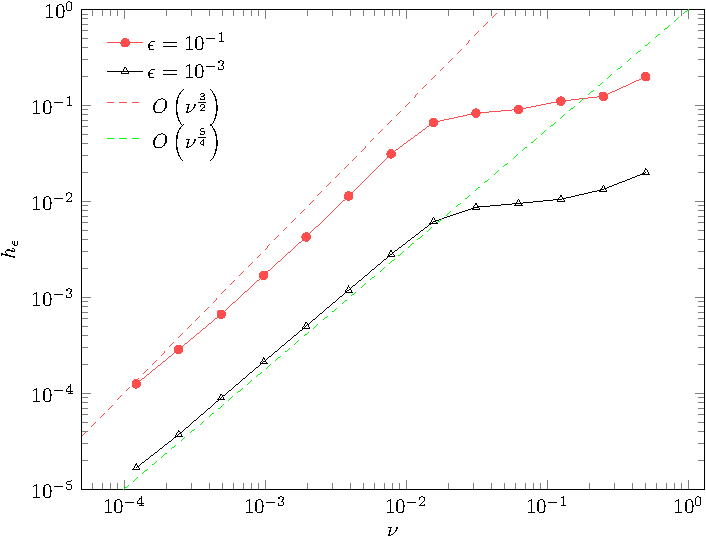
\includegraphics[height=0.32\textwidth]{pics_frequency_domain/h_nu.pdf}
&
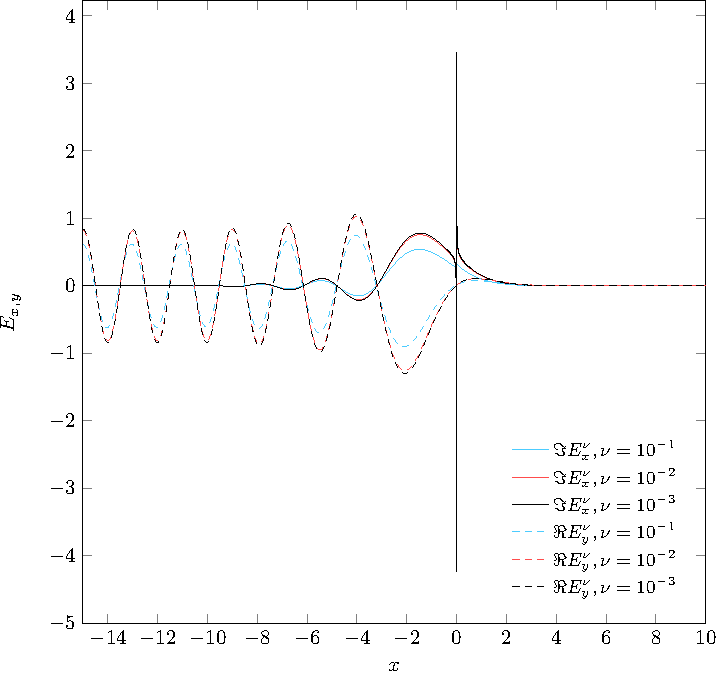
\includegraphics[height=0.32\textwidth]{pics_frequency_domain/res_sol.pdf}
\end{tabular}
\caption{We consider the problem (\ref{eq:main_frequency_domain}) with the parameters 
defined in Table \ref{tab:parameters}. In the left figure the dependence of $h_{\epsilon}$ as defined by (\ref{eq:def_epsilon}) on $\nu$ is demonstrated.  
In the right figure we show the computed solutions for this problem (\urev{for brevity denoted by $E_{x,y}^{\nu}$}) for different values of $\nu$. }
\label{fig:dependence}
\end{figure}
We can see that the estimate (\ref{eq:estimate_h}) is pessimistic compared to the one suggested by (\ref{eq:def_epsilon}), 
at least for given values of $\epsilon$ and for a chosen range of $\nu>0$.
\begin{remark}
It can be shown that $\|E^{\nu}_{x}\|_{L^2}\leq \frac{C}{\sqrt{\nu}},\; C>0$, 
and thus the relative error control
\bealn
 \frac{\|E^{\nu}_{x}-E^{\nu,h}_{x}\|_{L^2}}{\|E^{\nu}_{x}\|_{L^2}}\leq \epsilon
\eealn
 is ensured by choosing $h$ as $\beta_{\epsilon}\nu^{\frac{3}{4}}$, \mrev{$\beta_{\epsilon}>0$.}
\end{remark}

In Figure \ref{fig:small_nu} we demonstrate the dependence of the condition number of the matrix of the system (\ref{eq:simple_system}) 
on $\nu$, for several values of $h$.
Remarkably, for $\nu=0$ the computed matrices are not singular. We do not know the exact reason for this.
As an additional illustration, we compare the solutions for very small $\nu$ and $\nu=0$ for different meshes in Fig.~\ref{fig:small_nu}. 
\begin{figure}[htb!]
\begin{tabular}{cc}
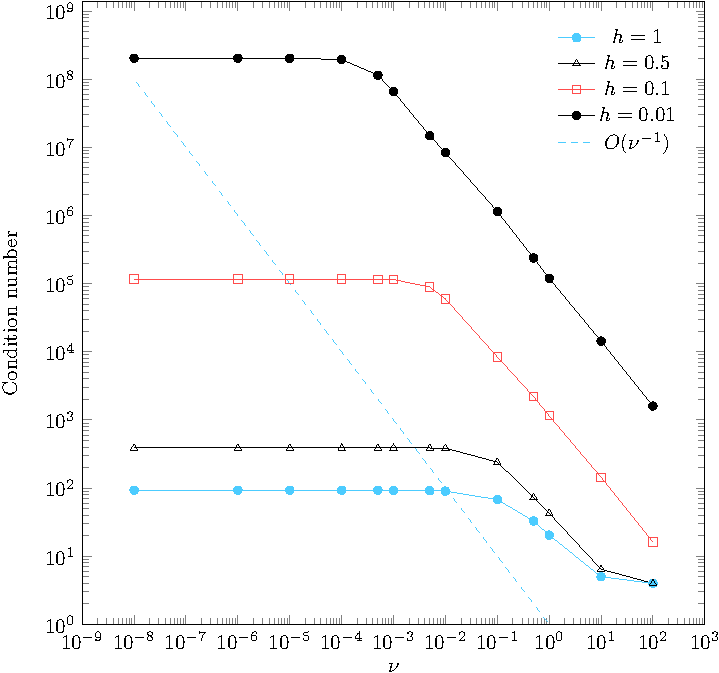
\includegraphics[height=0.32\textwidth]{pics_frequency_domain/fig_cond_num.pdf}&
 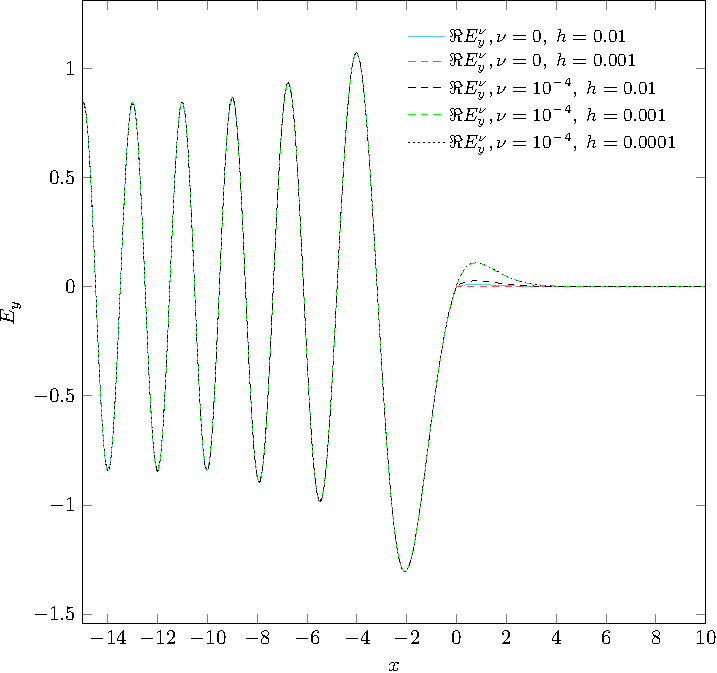
\includegraphics[height=0.32\textwidth]{pics_frequency_domain/ey_resonance.pdf}
 \end{tabular}
 \caption{
 We consider the problem (\ref{eq:main_frequency_domain}) with the parameters 
defined in Table \ref{tab:parameters}. The left plot demonstrates the dependence of the condition number of the system (\ref{eq:simple_system}) on $\nu$, for different values of $h$ (the condition 
 number for $\nu=0$ is not shown, however, for all values of $h$ as shown in the plot, the matrix was non-singular even for $\nu=0$). 
 The right plot shows \mrev{$E_{y}^{\nu,h}$} computed on different meshes for small $\nu$. It can be seen that for $h=10^{-2}$ and $h=10^{-3}$ the solutions 
 computed for $\nu=0$ are almost indistinguishable.}
 %It can be seen that for meshes that are coarse 
 %with respect to $\nu$ (e.g. $\nu=10^{-4}, \; h=10^{-2}$, or $\nu=0,\; h=10^{-2}$), the computed solution seems to be only piecewise-continuous in $\nu$, 
 %while for finer meshes and $\nu>0$ the solution seems to be smooth. }
 \label{fig:small_nu}
\end{figure}
%\begin{table}[ht!]
%\begin{tabular}{c|ccccccccc}
%\diagbox[width=10em]{$h$}{$\nu$}& 100 & 10 & 1 & 0.1 & 1e-2 & 1e-3 & 1e-4 & 1e-8 & 0\\
% \hline
%1 & 3.9634&4.3787 &4.987&36.949&42.394& 42.757 &42.79&42.793&42.793\\
%\hline
%0.5&      3.9931& 6.87&48.473 & 168.41  &207.34  & 209.63 & 209.83 & 209.85&  209.85\\
%\hline
% 0.1&      16.09  &     159.56  &     1146.1   &    8304.1   &     19169  &      20270   &     20344   &     20352   &     20352\\
% \hline
%0.05&      64.046  &     637.18  &     4686.2   &     38876 &  1.4e5 &  1.58e5 &   1.58e5 &  1.58e5 &  1.58e5\\
%\hline
% 0.01&       1600    &   15921 & 1.2e5  & 1.1e6 & 8.3e6  & 1.8e7   & 1.93e7  & 1.93e7  & 1.93e7\\
%\end{tabular}
%\caption{The condition number of the matrix of the system (\ref{eq:simple_system}) for different values of $\nu$ and $h$. }
%\label{tab:cond_number}
%\end{table}


\FloatBarrier

\subsection{A validation of the semi-lagrangian scheme}

We show the results of very basic simulations that the numerical strategy 
based on co-localised semi-lagrangian discretization is valid even for the resonant 
case.
The numerical tests have been kept to a minimum since \arev{many more} are needed to fully validate
the concept.

The setting of the numerical results of figure \ref{fig:vasl}
is the following. We use a 7th order semi-lagrangian scheme, and the CFL is $\nu=0.5$.
The \arev{peak} is the hybrid resonance, visible on $E_x$ and $u_x$.
The total energy $\mathcal E(t)$ is the physical energy. 
The comparison with figures \ref{fig:dependence} and \ref{fig:resonance_nus_ey_x} show that the 
singular nature of the \arev{resonance} is captured by this new scheme without any doubt.

\begin{figure}{h}
	\begin{center}
		\begin{tabular}{ccc}
			\includegraphics[angle=-90,width=5.cm]{pics_semilagrange/Ey_moit.eps}
			&
			\includegraphics[angle=-90,width=5.cm]{pics_semilagrange/Hz_moit.eps} &
			\includegraphics[angle=-90,width=5.cm]{pics_semilagrange/Ex_moit.eps}
			\\
			$E_y$ & $H_z$  & $E_x^\nu$ \\
			%\hline
			\hline
			\includegraphics[angle=-90,width=5.cm]{pics_semilagrange/uy_moit.eps}
			&
			\includegraphics[angle=-90,width=5.cm]{pics_semilagrange/normes_moit.eps}
			&
			\includegraphics[angle=-90,width=5.cm]{pics_semilagrange/ux_moit.eps}
			\\      
			$u_y$ & $t\mapsto \mathcal E(t)$ & $u_x^\nu$  \\
			
			%\includegraphics[width=4.cm]{cap14.png} 
			\\
			
			
		\end{tabular}   \end{center}
		\caption{An antenna sends a time harmonic wave on the left. The medium is propagative
			on the left and non propagative
			on the right. The resonance is visible on $E_x$ and $u_x$. The time of the simulation is $T=2000$. The number of cells
			is typically 10000 to reach convergence.}
		\label{fig:vasl}
	\end{figure}


%\subsubsection{No-Resonance Case}
%We choose the parameters so that in the frequency domain, for the limiting amplitude problem, $\hat{E}_{2}$ satisfies 
%the Airy equation \cite{}. 

%We set $\omega_c=0$ (thus $\delta(x)=0$), $\omega=1$ (hence $\alpha(x)=1-N_e(x)$), 
%choose the domain as $[-0.5, 10]$ and set the electron density $N_e(x)=1+x$. Importantly, $N_e(x)>0$ on the whole interval.
%The boundary conditions in (\ref{eq:bcs}) are chosen as $G=Ai'(0.5)$. 
%In all the experiments in this section the CFL number was chosen to be equal to 0.5.


%First let us fix $\nu=1e-2$. 
%To demonstrate that the limiting amplitude principle indeed holds, we fix a point $x=x_c$ 
%inside the domain $(-L,\; H)$ and plot the dependence of the solution $E_{y}^{\nu}(x_c,t), \; \hat{E}_2^{\nu}(x_c)\mathrm{e}^{it}$ 
%on time $t$ for a range of $t\gg 1$ in Figure \ref{fig:nu1e2_harmon}.  